\documentclass[10pt]{beamer}
\usetheme{Madrid}
\usepackage[utf8]{inputenc}
\usepackage[T1]{fontenc}\usepackage{helvet}\usepackage{courier}
\usepackage{amsmath,amssymb,booktabs,listings,tikz}
\usetikzlibrary{arrows.meta,positioning}
\logo{\includegraphics[height=6mm]{logo.png}}
\title{Kvantuminformatika -- 3. előadás}
\author{Teszt Elek}
\date{2026. ősz}
\lstset{basicstyle=\ttfamily\small,language=Python,keywordstyle=\color{blue}}
\begin{document}
\begin{frame}\titlepage\end{frame}

\begin{frame}{Qubit állapota}
Egy qubit állapota a $\mathbb{C}^2$ tér egységvektora:
\[ |\psi\rangle = \alpha|0\rangle + \beta|1\rangle, \qquad |\alpha|^2 + |\beta|^2 = 1 . \]
\begin{itemize}
\item<1-> A mérés valószínűségei: $P(0) = |\alpha|^2$, $P(1)=|\beta|^2$.
\item<2-> Bloch-gömb: $|\psi\rangle = \cos\frac{\theta}{2}|0\rangle + e^{i\varphi}\sin\frac{\theta}{2}|1\rangle$.
\item<3-> Sűrűségmátrix: $\rho = \sum_i p_i |\psi_i\rangle\langle\psi_i|$, $\operatorname{Tr}\rho = 1$.
\end{itemize}
\end{frame}

\begin{frame}{Hadamard-kapu (beillesztett képlet)}
A Hadamard-kapu mátrixa és hatása:
\begin{center}\includegraphics[width=0.8\textwidth]{formula.png}\end{center}
Kétszer alkalmazva az identitást kapjuk.
\end{frame}

\begin{frame}{Animált ábra}
\only<1>{\includegraphics[width=0.6\textwidth]{plotA.png}\\ Az első lépésben a szinusz.}
\only<2>{\includegraphics[width=0.6\textwidth]{plotB.png}\\ A második lépésben a koszinusz.}
\end{frame}

\begin{frame}{Áramkör}
\begin{center}
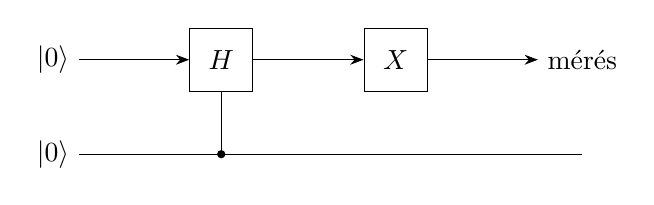
\begin{tikzpicture}[node distance=14mm, box/.style={draw, minimum size=8mm}]
\node (a) {$|0\rangle$}; \node[box, right=of a] (h) {$H$}; \node[box, right=of h] (x) {$X$}; \node[right=of x] (m) {mérés};
\draw[-{Stealth}] (a) -- (h); \draw[-{Stealth}] (h) -- (x); \draw[-{Stealth}] (x) -- (m);
\node[below=6mm of a] (b) {$|0\rangle$}; \fill (h |- b) circle (1.5pt); \draw (b) -- (m |- b); \draw (h |- b) -- (h);
\end{tikzpicture}
\end{center}
Az áramkör egy Bell-állapotot állít elő.
\end{frame}

\begin{frame}{Két hasáb}
\begin{columns}[t]
\begin{column}{0.48\textwidth}
\begin{itemize}\item Klasszikus bit: 0 vagy 1\item Determinisztikus\item Másolható\end{itemize}
\end{column}
\begin{column}{0.48\textwidth}
\begin{itemize}\item Qubit: szuperpozíció\item Valószínűségi mérés\item Nem klónozható\end{itemize}
\end{column}
\end{columns}
\end{frame}

\begin{frame}{Kapuk táblázata}
\begin{tabular}{lll}\toprule Kapu & Mátrix & Hatás \\ \midrule
$X$ & $\begin{pmatrix}0&1\\1&0\end{pmatrix}$ & bitcsere \\
$Z$ & $\begin{pmatrix}1&0\\0&-1\end{pmatrix}$ & fáziscsere \\ \bottomrule\end{tabular}
\end{frame}

\begin{frame}[fragile]{Szimuláció}
\begin{lstlisting}
import numpy as np
H = np.array([[1, 1], [1, -1]]) / np.sqrt(2)
psi = H @ np.array([1, 0])
print(abs(psi) ** 2)   # [0.5 0.5]
\end{lstlisting}
A kimenet a két mérési valószínűség.
\end{frame}

\begin{frame}{Összefoglalás}
\begin{itemize}\item A qubit állapota egységvektor.\pause \item A kapuk unitér mátrixok.\pause \item A mérés valószínűségi.\end{itemize}
\end{frame}
\end{document}
